\documentclass[12pt,a4paper,oneside]{article}

\usepackage[utf8]{inputenc}
\usepackage[portuguese]{babel}
\usepackage[T1]{fontenc}
\usepackage{amsmath}
\usepackage{amsfonts}
\usepackage{amssymb}
\usepackage{graphicx}

\usepackage{xcolor}
% Definindo novas cores
\definecolor{verde}{rgb}{0.25,0.5,0.35}
\definecolor{jpurple}{rgb}{0.5,0,0.35}
% Configurando layout para mostrar codigos Java
\usepackage{listings}
\lstset{
  language=Java,
  basicstyle=\ttfamily\small, 
  keywordstyle=\color{jpurple}\bfseries,
  stringstyle=\color{red},
  commentstyle=\color{verde},
  morecomment=[s][\color{blue}]{/**}{*/},
  extendedchars=true, 
  showspaces=false, 
  showstringspaces=false, 
  numbers=left,
  numberstyle=\tiny,
  breaklines=true, 
  backgroundcolor=\color{cyan!10}, 
  breakautoindent=true, 
  captionpos=b,
  xleftmargin=0pt,
  tabsize=4,
  escapeinside=||
}

\author{\\Universidade Federal de Jataí (UFJ)\\Bacharelado em Ciência da Computação \\Inteligência Artificial \\Esdras Lins Bispo Jr.}

\title{\sc \huge Primeira Prova}

\begin{document}

\maketitle

{\bf ORIENTAÇÕES PARA A RESOLUÇÃO}

\begin{itemize}
	\item A avaliação é individual, sem consulta;
	\item A pontuação máxima desta avaliação é 10,0 (dez) pontos, sendo uma das 04 (quatro) componentes que formarão a média final da disciplina: duas provas, um projeto e exercícios;
	\item A média final será calculada pela média ponderada das quatro supraditas notas [em que a primeira prova tem peso 40 (quarenta), a segunda prova tem peso 30 (trinta), o projeto tem peso 30 (trinta) e os exercícios-bônus são adicionados à media final];
	\item O somatório da pontuação de todas as questões desta avaliação é 11,0 (onze) pontos. Isto é um sinônimo de tolerância na correção. Se você por acaso perder 1,5 (um e meio), sua nota será 9,5 (nove e meio);
	\item O conteúdo exigido compreende os seguintes pontos apresentados no Plano de Ensino da disciplina: (1) Introdução à Inteligência Artificial, (2) Agentes Inteligentes, (3) Resolução de Problemas por meio de Busca, (5) Redes Neurais Artificiais, e  (6) Computação Natural.
\end{itemize}

\begin{center}
	\fbox{\large Nome: \hspace{10cm}}
	\fbox{\large Assinatura: \hspace{9cm}}
\end{center}

\newpage

\begin{enumerate}


	\item[] \colorbox{black}{
		\color{white}Todas as questões necessitam não apenas
	}\\ 
	\colorbox{black}{
		\color{white} serem respondidas, mas também justificadas.
	}

	\item (2,0 pt) {\bf [Russel 1.11 Adaptado]} ``Sem dúvida, os computadores não podem ser inteligentes - eles só podem fazer o que seus programadores determinam''. Esta última afirmação é verdadeira e implica a primeira? Justifique sua resposta baseado na discussão sobre as várias definições de Inteligência Artificial.
	
	\vspace*{0.3cm}
	
	{\color{blue} 
		{\bf Resposta:} A última afirmação é verdadeira: ``os computadores só podem fazer o que seus programadores determinam''. Mas não necessariamente implica a primeira. Isto acontece devido às várias concepções que podemos ter sobre o que é ser inteligente.
		
		Por exemplo, se a sua definição de inteligência for o grau de semelhança que o computador tem com a inteligência humana, temos pelo menos duas perspectivas a considerar. 
		
		A primeira perspectiva pode ser mais materialista, admitindo de certa forma que ``os seres humanos são máquinas determinadas pela sua matéria''. Nesta perspectiva, a última afirmação não implica a primeira.
		
		Porém, em uma segunda perspectiva não-materialista, pode-se admitir que ``os seres humanos são compostos por estruturas que vão além da matéria'' e, logo, não são necessariamente determinísticos. Assim, a última afirmação implica a primeira.
	}
			
	\item (2,0 pt) {\bf [ENADE 2008]} Julgue os itens a seguir, relativos a métodos de busca com informação (busca heurística) e sem informação (busca cega), aplicados a problemas em que todas as ações têm o mesmo custo, o grafo de busca tem fator de ramificação finito e as ações não retornam a estados já visitados.
	
		\begin{enumerate}
		\item[] I - A primeira solução encontrada pela estratégia de busca em largura é a solução ótima. 
		{\color{blue} VERDADEIRO. }
		\item[] II - A primeira solução encontrada pela estratégia de busca em profundidade é a solução ótima. \\
		{\color{blue} FALSO, pois a solução ótima pode estar em níveis acima da primeira solução encontrada, em nós que ainda não foram visitados.}
		\item[] III - As estratégias de busca com informação usam funções heurísticas que, quando bem definidas, permitem
		melhorar a eficiência da busca. {\color{blue} VERDADEIRO. }
		\item[] IV - A estratégia de busca gulosa é eficiente porque expande apenas os nós que estão no caminho da
		solução.\\
		{\color{blue} FALSO, pois embora ela expande apenas os nós que estão (aparentemente) no caminho da solução, ela não é a opção mais eficiente. A busca A* é um opção melhor, por exemplo.}
	\end{enumerate}
	
	Estão certos apenas os itens:
	
	\begin{enumerate}
		\item I e II.
		\item I e III. {\color{blue} Resposta correta.}
		\item I e IV.
		\item II e IV.
		\item III e IV.
	\end{enumerate}
	
	 \item (2,0 pt) {\bf [Russel 2.6 Adaptado]} Pode haver mais de um programa de agente que implemente uma
	dada função de agente? Dê um exemplo ou mostre por que não é
	possível.
	
	\vspace*{0.3cm}
	
	{\color{blue} 
		{\bf Resposta:} Sim, é possível. O programa de agente depende diretamente da arquitetura do agente que está disponível. Por exemplo, se a função de agente fosse uma função do tipo $f(p) = \sqrt{p}$, a arquitetura determinará os possíveis programas de agentes que podem ser implementados. Se a arquitetura não der um suporte a variáveis do tipo ponto-flutuante (por exemplo), e suportar apenas valores inteiros, será necessário utilizar alguma política de truncamento de valores para o resultado da função. Logo restrições na arquitetura do agente limita a diversidade de programa de agentes possíveis.
	}
	
	\item (2,0 pt)  Explique por quê o Perceptron pode executar as funções lógicas AND, OR e NOT, mas não resolve o OU-EXCLUSIVO (XOR).
	
	\vspace*{0.3cm}
	
	{\color{blue} {\bf Resposta:} O Perceptron consegue estabelecer um discriminante linear na base de exemplos utilizada. As três funções AND, OR e NOT podem ser separadas apenas por uma reta. Entretanto, a função XOR necessitaria no mínimo de duas retas para realizar a separação (o que não é suportado pelo Perceptron).
	\begin{center}
		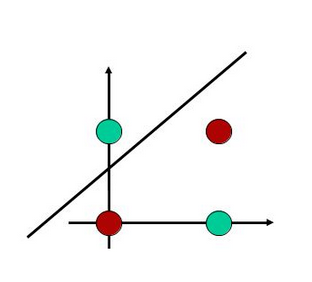
\includegraphics[width=0.5\textwidth]{images/xor}
	\end{center}
	}
	
	\item (3,0 pt) O grafo abaixo mostra a ligação entre 5 cidades e as respectivas distâncias em quilômetros:
	
	\begin{center}
		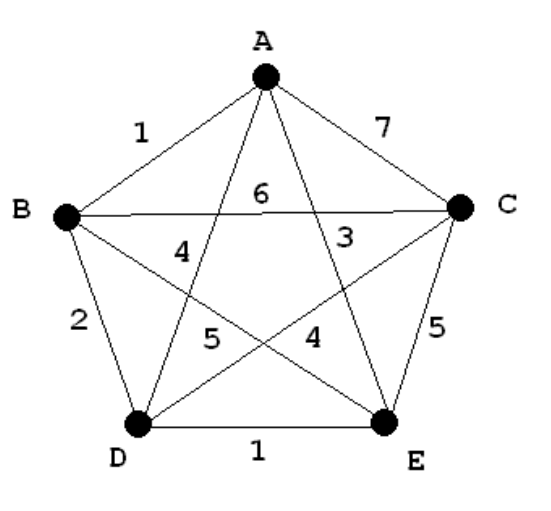
\includegraphics[width=5cm]{images/fig02.png}
	\end{center}
	
	Tem-se um problema em que é necessário passar por todas as cidades, apenas uma vez. O objetivo é encontrar uma rota de menor custo usando um algoritmo genético.
	
	\begin{enumerate}
		\item (0,5 pt) Proponha uma maneira de codificar os cromossomos.\\
		{\color{blue} {\bf Resposta:} Pode ser um 5-upla de forma em que cada elemento seja um gene do cromossomo. Cada gene representa uma cidade. É necessário garantir que não haja cidades repetidas.}
		\item (0,5 pt) Defina uma função de aptidão para avaliar a qualidade dos cromossomos.\\
		{\color{blue} {\bf Resposta:} Seja $d(c)$ o comprimento do percurso associado ao cromossomo $c$. A função de aptidão $f$ pode ser descrita a seguir:
			\begin{center}
				$f(c) = 35 - d(c)$
			\end{center}
			Assim, garantimos que quanto maior $f(c)$ for, mais apto será o cromossomo $c$.}
		\item (0,5 pt) Gere dois cromossomos e avalie a aptidão deles.\\
		{\color{blue} {\bf Resposta:} Sejam dois cromossomos $c_1 = (A,B,C,D,E)$ e $c_2 = (E,D,B,C,A)$. As aptidões de $c_1$ e $c_2$ são dadas a seguir:
			\begin{center}
				$f(c_1)$ 	= 35 - 12 = 23\\
				$f(c_2)$ 	= 35 - 16 = 19
		\end{center}}
		\item (0,5 pt) Realize o cruzamento entre os cromossomos.\\
		{\color{blue} {\bf Resposta:} Admita que foi sorteado que o ponto de corte seja entre os genes 3 e 4. Logo temos os dois cromossomos filhos $f_1$ e $f_2$:
			\begin{center}
				$c_1 = (A,B,C||D,E)$\\
				$c_2 = (E,D,B||C,A)$\\
				temos\\
				$f_1 = (A,B,C,\fbox{C,A}) \rightarrow (A,B,D,C,E)$\\
				$f_2 = (E,D,B,\fbox{D,E}) \rightarrow (E,C,B,D,A)$\\
			\end{center}
			Após o cruzamento, foi necessária realizar adaptações para que o cromossomo gerado fosse um cromossomo válido. Para isto, foi necessário garantir que 
			\begin{itemize}
				\item[] (i) havendo repetições de genes, um dos genes deve ser substituído por uma cidade ainda não presente, e
				\item[] (ii) o cromossomo gerado não pode ser igual a um dos pais.
		\end{itemize}}
		\item (0,5 pt) Aplique uma mutação em um gene dos cromossomos.\\
		{\color{blue} {\bf Resposta:} Admita que foi sorteado o gene 2 de $c_1$ e o gene 4 de $c_2$. Para que os cromossomos mutantes $m_1$ e $m_2$ sejam válidos, será realizada uma permutação de seus genes. Suponha também que os genes 1 e 2 participarão da permutação em $c_1$ e $c_2$, respectivamente:
			\begin{center}
				$c_1 = (A,B,C,D,E)$\\
				$c_2 = (E,D,B,C,A)$\\
				temos\\
				$c_1 = (\underline{A},\fbox{B},C,D,E) \rightarrow (B,A,C,D,E)$\\
				$c_2 = (E,\underline{D},B,\fbox{C},A) \rightarrow (E,C,B,D,A)$
		\end{center}}
		\item (0,5 pt) Aplique a função de aptidão nos descendentes gerados verificando se a solução encontrada é melhor ou não.\\
		{\color{blue} {\bf Resposta:} As aptidões de $f_1$, $f_2$, $m_1$ e $m_2$ são dadas a seguir:
			\begin{center}
				$f(f_1)$ 	= 35 - 12 = 23\\
				$f(f_2)$ 	= 35 - 17 = 18\\
				$f(m_1)$ 	= 35 - 13 = 22\\
				$f(m_2)$ 	= 35 - 17 = 18
			\end{center}
			Os cromossomos $f_1$ e $m_1$ têm valor de aptidão próximo ou igual ao valor de $c_1$. Já os cromossomos $f_2$ e $m_2$ são menos aptos do que os seus genitores.}
		\end{enumerate}
\end{enumerate}
\end{document}